\documentclass[10pt,twocolumn,letterpaper]{article}

\usepackage{cvpr}
\usepackage{times}
\usepackage{epsfig}
\usepackage{graphicx}
\usepackage{amsmath}
\usepackage{amssymb}
% Include other packages here, before hyperref.

% If you comment hyperref and then uncomment it, you should delete
% egpaper.aux before re-running latex.  (Or just hit 'q' on the first latex
% run, let it finish, and you should be clear).
%\usepackage[breaklinks=true,bookmarks=false]{hyperref}

\cvprfinalcopy % *** Uncomment this line for the final submission

\def\cvprPaperID{****} % *** Enter the CVPR Paper ID here
\def\httilde{\mbox{\tt\raisebox{-.5ex}{\symbol{126}}}}
% Pages are numbered in submission mode, and unnumbered in camera-ready
%\ifcvprfinal\pagestyle{empty}\fi
\setcounter{page}{1}
\begin{document}

%%%%%%%%% TITLE
\title{Freddie Mac Machine Learning}

\author{Thomas Billman}
% For a paper whose authors are all at the same institution,
% omit the following lines up until the closing ``}''.
% Additional authors and addresses can be added with ``\and'',
% just like the second author.
% To save space, use either the email address or home page, not both

\maketitle
%\thispagestyle{empty}

%%%%%%%%% ABSTRACT

%%%%%%%%% BODY TEXT
\section{Introduction}

Freddie Mac holds a large portion of the United States of America's home mortgages. As such looking for trends in the values and performance of these loans is crucial. Our dataset consists of data collected at the time loans were issued and a calculated Net Present Value (NPV) that acts as a proxy for the total value of each loan. This paper summarizes a subset of the different variables found in the dataset. The dataset can be found on my GitHub at the following address:
https://tinyurl.com/ycpr8lrj

%-------------------------------------------------------------------------
\section{Logistic Regression}
We begin our further analysis by predicting whether the NPV of an observation will be positive or negative. The covariates considered include Credit Score, Mortgage Insurance, Debt to Income ratio, among others. This model predicted that every mortgage would have a positive NPV, so it's accuracy measures were as follows:
\begin{center}
\begin{tabular}{ |c|c| } 
	\hline
	Sensitivity & 1 \\ 
	\hline
	Specificity & 0 \\
	\hline
	Accuracy & 0.98125\\ 
	\hline
\end{tabular}
\end{center}

Additionally the ROC Curve can be found in Figure \ref{fig:ROC}. The area under the curve was .6417, which is not very significant.

\section{Linear Discriminant Analysis}

We continue by applying Linear Discriminant Analysis. These results were the same as logistic regression, by predicting all rows as positive NPV. 
\begin{center}
	\begin{tabular}{ |c|c| } 
		\hline
		Sensitivity & 1 \\ 
		\hline
		Specificity & 0 \\
		\hline
		Accuracy & 0.98125\\ 
		\hline
	\end{tabular}
\end{center}

\section{Quadratic Discriminant Analysis}

Quadratic Discriminant Analysis begins predicting NPVs that are not all positive. The table of results is as follows:

\begin{center}
	\begin{tabular}{ |c|c|c| } 
		\hline
		 & True - & True +\\ 
		\hline
		Predicted - & 246 & 1587 \\ 
		\hline
		Predicted + & 3676 & 203619\\
		\hline
	\end{tabular}
\end{center}

This yields the following sensitivity, specificity, and accuracy:
\begin{center}
	\begin{tabular}{ |c|c| } 
		\hline
		Sensitivity & 0.9922663 \\ 
		\hline
		Specificity & 0.0627231 \\
		\hline
		Accuracy & 0.9748336\\ 
		\hline
	\end{tabular}
\end{center}

It is worth noting that although a specificity of .06 seems poor, it is nearly 3 times more accurate than random guessing.


\section{KNN Analysis}

We continue through to KNN analysis, which produced even better specificity than QDA. This was the resulting confusion matrix:

\begin{center}
	\begin{tabular}{ |c|c|c| } 
		\hline
		& True - & True +\\ 
		\hline
		Predicted - & 601 & 209 \\ 
		\hline
		Predicted + & 3321 & 204997\\
		\hline
	\end{tabular}
\end{center}
This yields the following sensitivity, specificity, and accuracy:
\begin{center}
	\begin{tabular}{ |c|c| } 
		\hline
		Sensitivity & 0.1532381 \\ 
		\hline
		Specificity & 0.9989815 \\
		\hline
		Accuracy & 0.9831204 \\ 
		\hline
	\end{tabular}
\end{center}

Of the four methods tested this had the best accuracy and impressive specificity for this dataset. 


\section{Cross Validated Results}

We repeat the above methods using 5-fold cross validation.

\subsection{Logistic Regression}
Overall average accuracy was 0.981719 and took ~15 seconds to run. All sensitivities were 1 and all specificities were 0.

\subsection{LDA Analysis}
Overall average accuracy was 0.9812459  and took ~5 seconds to run. All sensitivities were 1 and all specificities were 0.

\subsection{QDA Analysis}
Overall average accuracy was 0.9747953 and took ~ 4 seconds to run. All sensitivities were ~ .992 and specificities were between .049 and .075.

\subsection{KNN Analysis}
Overall average accuracy was 0.9806004 and took ~ 9 minutes to run. All sensitivities were ~ .998 and specificities were between .077 and .087.


\section{Conclusion}
These models show that QDA and KNN were better classifiers for our data than logistic or LDA. Additionally, cross validated results show lower accuracies than testing on your training data. However, this is to be expected.


\begin{figure}
	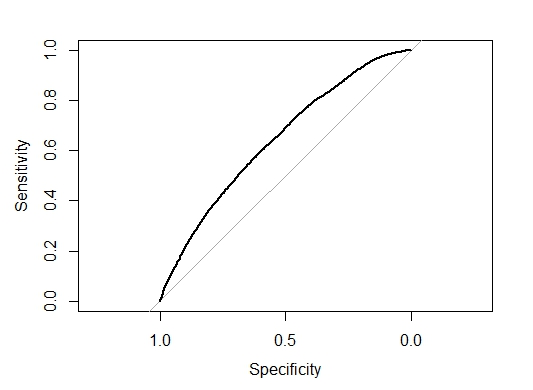
\includegraphics[width=0.45\textwidth]{images/ROC}
	\caption{ROC Curve for Logistic Regression}
	\label{fig:ROC}
\end{figure}


\end{document}
